% Lezione 1/2024-02-26
% - Introduzione filosofica alla fisica (di che si occupa, rapporto con la realta' e filosofia della quantificazione, metodo scientifico)
% - Quantificazione: misura ed errore di misura, stima

% Lezione 2/2024-02-28
% - Notazioni sulla quantificazione: ordine di grandezza
% (include altri argomenti, ma con un capitolo dedicato)
% - Introduzione alla descrizione quantitativa del moto (cinematica?)
% - cinematica del punto materiale da una a piu' dimensioni: moto rettilineo uniforme, piano cartesiano
% - equazioni del moto, con notazione vettoriale
% Esercitarsi su: moto rettilineo uniforme, vettori e trigonometria, sistemi di riferimento cartesiani e algebra sul piano cartesiano

% Lezione 3/2024-03-04
% - introduzione alla dinamica
% - prima e seconda legge
% - esercizi su moto uniformemente accelerato
% - accenni al concetto di forza e introduzione alla forza elastica con legge di hooke

% Lezione 4/2024-03-06
% - grafico orario: grafico nel quale un asse riporta lo spazio (una dimensione), mentre sull'altro il tempo
% - differenza tra SPOSTAMENTO e distanza
% - interpretazione grafica della velocità e accelerazione, con analisi di funzione

% Lezione 5/2024-03-11
% - moto del punto nel piano
% - sistema di riferimento con vettore posizione
% - accelerazione in moti con traiettoria curvilinea
% - la STATICA si occupa della quiete

\documentclass{book}

\usepackage{feynmanslop}

\title{Fisica}
\author{Zeno Saletti}
\date{\today}


\begin{document}


\begin{titlepage}

\maketitle

\epigraph{If, in some cataclysm, all of scientific knowledge were
to be destroyed, and only one sentence passed on to the next generations
of creatures, what statement would contain the most information in the
fewest words? I believe it is the \textit{atomic hypothesis} [...]
that \textit{all things are made of atoms—little particles that move
around in perpetual motion, attracting each other when they are a little
distance apart, but repelling upon being squeezed into one another.}
In that one sentence, you will see, there is an enormous amount of
information about the world, if just a little imagination and
thinking are applied.}{Richard P. Feynman,\\\textit{The Feynman Lectures on Physics}}

\vspace*{9cm}
\begin{center}
Consigliamo di consultare questa dispensa ascoltando il brano seguente:\\
\href{https://www.youtube.com/watch?v=JuSsvM8B4Jc}{\textcolor{blue}{\textit{Cornfield Chase} by Hans Zimmer (from \textit{Interstellar})}}
\end{center}

\end{titlepage}

\dominitoc %otherwise tocs won't appear
\tableofcontents

\part{Book}

% Lezione 1/2024-02-26
% - Introduzione filosofica alla fisica (di che si occupa, rapporto con la realta' e filosofia della quantificazione, metodo scientifico)
% - Quantificazione: misura ed errore di misura, stima

% Lezione 2/2024-02-28
% - Notazioni sulla quantificazione: ordine di grandezza
% (include altri argomenti, ma con un capitolo dedicato)

\chptr{Introduzione alla Fisica}

\section{Definizione e scopi della fisica}

Si possono formulare definizioni diverse riguardo la disciplina scientifica
della fisica, come la seguente:

\vspace{8pt}
\begin{tcolorbox}[colback = yellow!30, colframe = yellow!30!black, title = {Fisica}]
La fisica è lo studio quantitativo delle leggi fondamentali della natura, cioè
delle leggi che governano tutti i fenomeni naturali dell'universo.

Una legge fisica è una regolarita' della natura esprimibile in forma matematica.
\end{tcolorbox}
\vspace{5pt}

La fisica si avvale del \textbf{metodo scientifico}, secondo cui la natura deve
essere interrogata per vie sperimentali, facendosi guidare da \textbf{ipotesi} e
modelli teorici. Una particolarita' di questo metodo è la capacita' di isolare
un certo fenomeno che si intende studiare, tralasciando (si usera' spesso il
termine \textit{trascurare}) certi aspetti ritenuti non rilevanti in modo da
scoprire quelle regolarita' dalle quali potrebbe essere dedotta una certa'
relazione matematica.

Il ruolo della matematica è di fornire un linguaggio formale per descrivere
quantitativamente i fenomeni osservati e costruire modelli utili alla loro
trattazione.



\section{Grandezze fisiche}
La fisica è una scienza quantitativa, ovvero essa si occupa di caratteristiche
e proprieta' del mondo che possono essere misurate e quantificate: le cosiddette
grandezze fisiche. Esempi di grandezze fisiche sono la lunghezza, la massa, la
temperatura, la durata temporale e cosi' via.

\vspace{8pt}
\begin{tcolorbox}[colback = yellow!30, colframe = yellow!30!black, title = {Grandezza fisica}]
Una grandezza fisica è una caratteristica di un oggetto o di un fenomeno che puo'
essere misurata in termini quantitativi (oltre che oggettivi, ovvero indipendentemente
dalle sensazioni personali degli individui).
\end{tcolorbox}
\vspace{5pt}

È implicito, intuitivamente, il concetto di \textbf{misura}. Misurare una grandezza
fisica significa confrontarla con una grandezza ``campione'', detta \textbf{unita'
di misura}, e stabilire quante volte l'unita' di misura è contenuta nella
grandezza data. Il valore numerico ottenuto è la misura della grandezza e deve
essere sempre accompagnato dall'unita' di misura.
In altre parole, la \textbf{misura} non è altro che un \textit{rapporto} tra la
grandezza che si intende misurare e la grandezza campione scelta convenzionalmente
per tale scopo.

Mostriamo un esempio: supponiamo di voler misurare la lunghezza di qualsiasi cosa
in ``chiavette USB'' (si potrebbe argomentare circa quale chiavetta si stia
impiegando e quale posizione la chiavetta debba assumere durante la misura.
Supponiamo qui che la chiavetta sia posta in verticale, senza perderci in ulteriori
dettagli). Decidiamo poi di misurare l'altezza di una porta—anche qui, non
specifichiamo quale porta—utilizzando l'unita' appena scelta. Supponiamo quindi
di aver registrato il seguente dato:
\[ H = 20 \text{ chiavette USB} \]
Notare come siano stati specificati:
\begin{itemize}
    \item Un nome per l'oggetto che si intendeva misurare, $H$, ovvero l'altezza
    della porta.
    \item Il valore numerico individuato, 20.
    \item Una affermazione per legare il nome e il dato, = (``corrisponde a'', ``è
    uguale a'')—caratteristica che peraltro si trova anche nei linguaggi di
    programmazione.
    \item L'unita' di misura, chiavette USB.
\end{itemize}
Tuttavia, tale misurazione non è stata affatto ``sincera'': non vi è la
garanzia del fatto che il valore registrato sia esatto. La prossima sezione
trattera' questo problema, ovvero quello dell'\textit{incertezza}.


\section{Incertezza}
Idealmente, si vorrebbe impiegare, grazie alle misure, numeri puntuali ed esatti.
In altre parole, dei numeri con una precisione indefinita, aventi un numero
illimitato di cifre decimali e non.

Ma quando si effettua una misura di una grandezza, il risultato ottenuto è noto solo
con una certa precisione. Riprendendo l'esempio della chiavetta USB, è impossible
misurare con certezza tutte le lunghezze, in quanto non multipli esatti della
chiavetta stessa: ci sara' sempre un certo margine di ``un pezzo di chiavetta'',
minore dell'unita' prescelta. Ma al di sotto di quella unita' non è possibile
fornire alcuna garanzia sulla puntualita' del dato. In altre parole, la
\textit{sensibilità}\footnote{La più piccola variazione della grandezza che lo
strumento è in grado di rilevare.} dello strumento è uno dei limiti alla precisione
della misura.

\vspace{8pt}
\begin{tcolorbox}[colback = yellow!30, colframe = yellow!30!black, title = {Cifre significative del risultato di una misura}]
Le cifre significative del risultato di una misura sono le cifre note
con certezza e la prima cifra incerta. In altre parole, esse sono le cifre che si
possono controllare con lo strumento impiegato nella misura.
\end{tcolorbox}
\vspace{5pt}

Ad esempio, il valore corrispondente alla lunghezza di una barca $L = 10,5$ m
possiede tre cifre significative, che non equivale a $10,50$ m. Il secondo dato,
infatti, dichiara che la misurazione è stata possibile controllando le cifre
fino al centimetro. $L = 0,002$ possiede solo una cifra significativa, perché
in genere si ignorano gli zeri a sinistra della prima cifra significativa diversa
da zero. Possono essere ambigui valori come $L = 2500 \text{ m}$: quali zeri sono
cifre significative? Come vedremo tra poco, è utile esprimere questi valori in
notazione scientifica per eliminare ambiguità.

Vi potrebbero anche essere errori dovuti a imprecisioni introdotte nell'utilizzo
degli strumenti di misura. Questo errore deve tuttavia essere quantificato ed ogni
misura ne è affetta (comprese quelle che non la riportano).

\vspace{8pt}
\begin{tcolorbox}[colback = yellow!30, colframe = yellow!30!black, title = {Risultato della misura di una grandezza}]
Il risultato della misura di una grandezza è sempre un'approssimazione
accompagnata da una certa incertezza, ovvero un \textbf{valore attendibile}
e un \textbf{errore assoluto} (o semplicemente \textit{incertezza}).
\[ x = \overline{x} \pm e_x  \]
\end{tcolorbox}
\vspace{5pt}

Questo risultato non è quindi altro che un intervallo in cui il valore reale
della misura si trova. Ci limiteremo agli errori relativi a singole misure,
nelle quali $x$ corrisponde al valore misurato e $e_x$ la sensibilità dello
strumento. Di conseguenza, possiamo ora correggere il risultato della misura
effettuata in chiavette USB:
\[ H = (20 \pm 1) \text{ chiavette USB} \]

\section{Notazione scientifica e ordini di grandezza}
Unità di misura come il metro e il kologrammo sono comode nella vita di tutti i
giorni, ma rappresentano quantità enormi su scala atomica e subatomica e quantità
minuscole su scala astronomica e cosmica. Conseguenza di ciò è che alcune misure
possono essere espresse da numeri ``scomodi''. Considerando solo valori attendibili,
la massa dell'atomo di idrogeno è circa
\[ m_H = 0,000 000 000 000 000 000 000 000 001 67 \text{ kg} \]
mentre la massa della Terra è
\[ m_T = 5 970 000 000 000 000 000 000 000 \text{ kg} \]
È pressoché evidente il motivo di tale scomodità: la notazione è di difficile
trattazione. Viene dunque in aiuto la \textbf{notazione scientifica}, ovvero una
notazione numerica che permette di contrarre rappresentazioni estese impiegando
potenze di 10. Nella notazione scientifica, ogni numero è scritto come prodotto
di due fattori:
\begin{itemize}
    \item Un numero decimale $x:x\in R, 1\leq x < 10$\footnote{In realtà, questa notazione corrisponde alla variante ``ingegneristica''. Esiste anche una notazione che prevede che il valore espresso $x$ sia $0\leq x < 1$.}.
    \item Una potenza di 10, con esponente intero.
\end{itemize}
Pertanto, le misure precedenti si possono esprimere in notazione scientifica come
segue:
\[ m_H = 1,67 \cdot 10^{-27} \text{ kg} \]
\[ m_T = 5,97 \cdot 10^{24} \text{ kg}\]
Notare come la notazione sia in grado di eliminare ambiguità sul numero di cifre
significative: ora sappiamo che la massa della Terra è stata calcolata fino a
tre cifre significative e non 25.

Non sempre è necessario calcolare esattamente il valore di una certa grandezza.
Talvolta basta averne solo un'idea approssimata. Supponiamo, ad esempio, che sia
sufficiente sapere se una certa massa vale all'incirca 1 grammo oppure 1
ettogrammo. In questo caso, possiamo accontentarci di stimare il valore della
massa con un'accuratezza di un fattore 10, cioè di calcolare il suo ordine di
grandezza.

\vspace{8pt}
\begin{tcolorbox}[colback = yellow!30, colframe = yellow!30!black, title = {Ordine di grandezza}]
L'ordine di grandezza di un numero è la potenza di 10 più vicina a quel numero.
\end{tcolorbox}
\vspace{5pt}

Per determinare l'ordine di grandezza di un numero occorre quindi esprimerlo in
notazione scientifica—prodotto di un numero decimale compreso tra 1 e 10 e di
una potenza di 10—e poi approssimare il valore alla potenza di 10 più vicina.
In particolare:
\begin{itemize}
    \item Se il numero decimale è minore di 5, si mantiene l'esponente della
    potenza. Ad esempio:
    \[ 3,6 \cdot 10^2 \to \text{ Ordine di grandezza } 10^2 \]
    \[ 4,2 \cdot 10^{-3} \to \text{ Ordine di grandezza } 10^{-3} \]

    \item Se il numero decimale è maggiore di 5, si somma +1 all'esponente della
    potenza. Ad esempio:
    \[ 9 \cdot 10^2 \approx 10 \cdot 10^2 \to \text{ Ordine di grandezza } 10^3 \]
    \[ 8,1 \cdot 10^{-12} \approx 10 \cdot 10^{-12} \to \text{ Ordine di grandezza } 10^{-11} \]
\end{itemize}


Sono stati definiti dei prefissi stadard per certi ordini di grandezza notevoli,
cioè quelli che, escludendo la potenza nulla, rappresentano multipli di tre.
Utilizzando questi prefissi, di fianco all'unità di misura adottata, si contrae
ancora di più la notazione scientifica, sottointendendo un certo ordine di
grandezza.

\marginpar{
    \footnotesize
    %\hspace*{-0.5cm}
    \begin{tabular}{c|c|c}
        Potenza   & Simbolo & Prefisso\\
        \hline
        $10^{12}$  & T       & Tera\\
        $10^{9}$   & G       & Giga\\
        $10^{6}$   & M       & Mega\\
        $10^{3}$   & k       & kilo\\
        $10^{-3}$  & m       & milli\\
        $10^{-6}$  & $\mu$   & micro\\
        $10^{-9}$  & n       & nano\\
        $10^{-12}$ & p       & pico\\
    \end{tabular}
}
\chptr{Descrizione del moto}
\marginpar{\minitoc}

\section{Moto del punto}
Un corpo è in moto quando la sua posizione cambia nel tempo. Nel descrivere il
moto, si introdurrà la seguente semplificazione: Gli oggetti saranno
trattati come \textit{punti materiali}, ovvero concentrati in un punto
adimensionale. In particolare, \textit{le dimensioni dell'oggetto del quale si
intende studiare il moto saranno considerate trascurabili rispetto a quelle
dell'ambiente circostante}.

\subsection{Posizione e traiettoria}
Alla base della descrizione del moto, è importante individuare quelli che sono
chiamati \textit{posizione} e \textit{traiettoria}. Avendo assunto la semplificazione
del punto materiale, è intuibile che la posizione verrà descritta matematicamente
come una tupla di coordinate inserite in un sistema di assi cartesiani. Tra le
coordinate, è importante tenere presente anche il tempo. Di fatto, abbiamo
introdotto il moto definendolo come variazione della posizione nel tempo.

La traiettoria non è altro che la linea che unisce le posizioni occupate
successivamente dal corpo. Tratteremo prima moti con traiettorie rettilinee,
per poi passare a traiettorie curvilinee semplici, come il moto circolare.

\subsection{Sistemi di riferimento}
Abbiamo detto che il moto è caratterizzato da un cambiamento di posizione. Il primo
passo nella descrizione del moto di un corpo consiste quindi nello stabilire il
modello da adottare per catturare il concetto di \textbf{posizione}. Sappiamo già
che i modelli della fisica si basano sul linguaggio matematico; il modello più
naturale che si possa adottare è dunque un sistema di assi cartesiani. Da qui, la
posizione del corpo può essere specificata mediante coordinate. Una speciale
coordinata è il tempo (in caso di moti in più di una dimensione spaziale, il
tempo viene spesso omesso dalla rappresentazione grafica).

\begin{marginfigure}
    \centering
    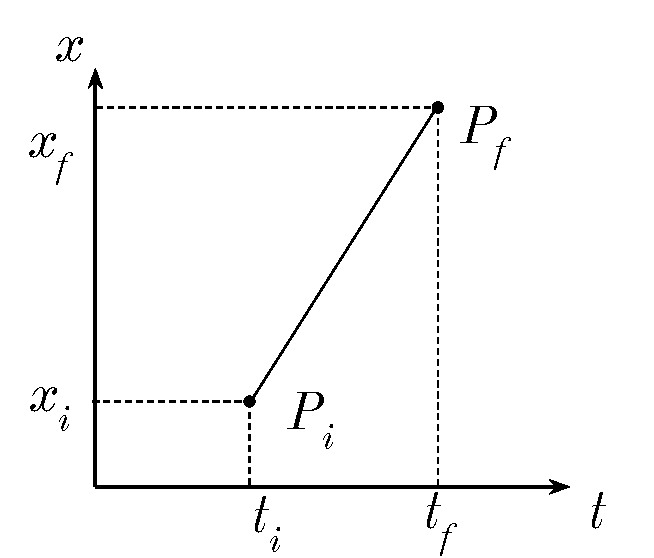
\includegraphics[width = \marginparwidth]{puntomateriale.pdf}
    \caption{Sistema di riferimento con una sola dimensione spaziale ($x$)
    in funzione del tempo ($t$). All'istante $t_i$, il punto materiale $P$
    si trova nella posizione $x_i$}
    \label{point}
\end{marginfigure}

La scelta del sistema di riferimento di assi cartesiani è del tutto arbitraria\footnote{
Gli assi possono addirittura non essere ortogonali, purché si segua la \textit{regola del
parallelogramma} e si rinunci alle proprietà e alle regolarità matematiche degli
assi ortogonali, come il teorema di Pitagora per il calcolo del modulo dei
vettori.}, ma una volta fissata è necessario essere coerenti con essa.
Questo permette di riflettere sul fatto che il moto è sempre relativo al sitema di
riferimento adottato: cambiando sistema di riferimento, il moto cambia.


\subsection{Distanza e spostamento}
Durante il moto, è possibile registrare la \textbf{distanza} percorsa
dall'oggetto e il suo \textbf{spostamento}. Il primo è una grandezza
scalare e corrisponde alla distanza totale percorsa durante il tragitto
effettuato dall'oggetto in moto. Il secondo è una grandezza vettoriale e
corrisponde al cambiamento di posizione,
cioè la differenza tra la posizione iniziale e quella finale dell'oggetto:
\[ \Delta \mathbf{x} = \mathbf{x}_f - \mathbf{x}_i \]


\section{Interpretazioni geometriche}

\begin{marginfigure}
    \centering
    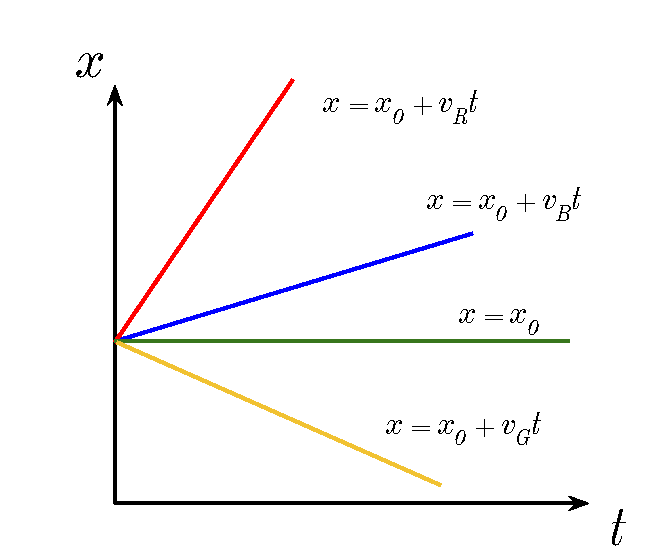
\includegraphics[width = \marginparwidth]{velocita.pdf}
    \caption{Oggetti in moto rettilineo uniforme con velocità differenti}
\end{marginfigure}


\section{Moto rettilineo uniforme}


\section{Accelerazione}



\section{Moto circolare}
Cambiamo ora la traiettoria dell'oggetto in moto, considerando quella circolare.
Per descrivere un moto circolare è conveniente impiegare coordinate differenti,
dette polari. Fissando il centro di un piano cartesiano al centro di una
circonferenza di raggio $r$, possiamo identificare la posizione di ogni punto
della circonferenza con la coppia $(r, \theta)$, dove $\theta$ è l'angolo
formato dalla semiretta appartenente al sistema di riferimento e dalla semiretta
che interseca la circonferenza nel punto desiderato (entrambe le semirette
hanno origine nel centro del piano cartesiano, quindi della circonferenza).

\begin{marginfigure}
    \centering
    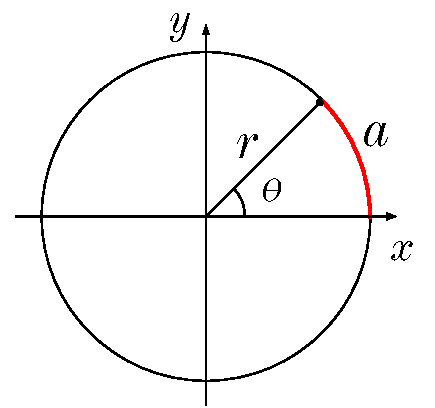
\includegraphics[width = \marginparwidth]{riferimentocirc.pdf}
    \caption{Sistema di riferimento per un moto circolare}
    \label{circref}
\end{marginfigure}

Assumeremo qui che $r$ non varia durante il moto. Per questo, viene omessa
la coordinata $r$ e si considera invece la posizione derivante da $\theta$,
detta anche \textit{posizione angolare}. Convenzionalmente, $\theta > 0$ se
misurato in senso antiorario a partire dall'asse di riferimento (come in
Figura \ref{circref}). Si utilizzano inoltre i \textit{radianti} per misurare
$\theta$. I radianti tornano infatti comodi, perché permettono di semplificare
le relazioni tra le grandezze in gioco durante il moto circolare. Innanzitutto,
dato l'arco $a$ in Figura \ref{circref}, vale la relazione \[ a = r\theta \]
Di fatto, la lunghezza totale della circonferenza corrisponde a $C = 2\pi r$,
dove $2\pi$ corrisponde ad un angolo giro espresso in radianti.

\subsection{Velocità angolare e velocità tangenziale}
Studiamo ora il cambiamento della posizione angolare nel tempo. Come per il
moto rettilineo, possiamo considerare il rapporto tra lo spostamento angolare
e l'intervallo di tempo trascorso. Da qui, si ottiene la velocità angolare:
\[ \omega = \frac{d\theta}{dt} \]
In ogni istante, una particella in moto circolare si muove in direzione
tangenziale alla traiettoria.
\begin{marginfigure}
    \centering
    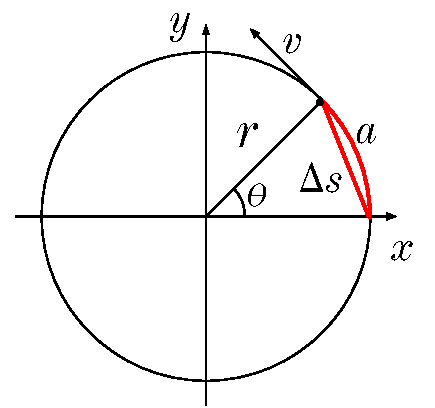
\includegraphics[width = \marginparwidth]{circspeed.pdf}
    \caption{Velocità tangenziale}
    \label{circspeed}
\end{marginfigure}
È chiaro che la particella, muovendosi, copre una certa distanza sulla
circonferenza in un dato intervallo di tempo. Possiamo quindi affermare
che essa ha una velocità, detta \textit{tangenziale}, $v$, oltre che
quella angolare $\omega$. Cerciamo una relazione tra esse: supponiamo che
la particella effettui, in un intervallo infinitesimo $\Delta t$, uno
spostamento angolare altrettanto piccolo $\Delta\theta$ come mostrato in
Figura \ref{circspeed}. Lo spostamento $\Delta s$, dato dalla corda che
sottende l'angolo $\Delta\theta$, approssima l'arco $a = r\Delta\theta$. Quindi:
\[ v = \lim_{\Delta t \to 0}\frac{\Delta s}{\Delta t} = \lim_{\Delta t \to 0} \frac{r\Delta\theta}{\Delta t} = r\lim_{\Delta t \to 0}\frac{\Delta\theta}{\Delta t} = r\omega \]
Abbiamo quindi ottenuto la relazione cercata:
\[ v = r\omega \]
Notare come $v\propto r$, al contrario di $\omega$. Ciò significa che,
assumendo una velocità angolare costante, la velocità tangenziale è tanto
maggiore quanto più $r$ cresce.

\subsection{Moto circolare uniforme}
Un moto circolare uniforme è un moto circolare con velocità \textit{angolare} costante.
Le regolarità di questo tipo di moto permettono di studiare altre grandezze
importanti per il moto circolare: periodi e accelerazioni.

\subsubsection*{Periodo e frequenza}
La particolarità di questo moto è la sua periodicità, perché esso si ripete
ciclicamente nel tempo. In particolare, un oggetto torna ad occupare la medesima
posizione iniziale dopo un certo intervallo di tempo, chiamato \textbf{periodo} ($T$):
in altre parole, il tempo necessario per compiere ``un giro (ciclo) completo''.
Nel nostro caso, un giro completo corrisponde all'intera circonferenza $C = 2\pi$.
Sapendo che $\omega = \frac{d\theta}{dt}$, è immediato ricavare il periodo:
\[ T = \frac{2\pi}{\omega} \]
Si impiega spesso anche la \textbf{frequenza}, che corrisponde al reciproco
del periodo:
\[ f = \frac{1}{T} \]
L'unità di misura è l'\textit{Hertz} (Hz), ovvero ``cicli al secondo'' (s$^{-1}$),
quindi il numero di cicli compiuti nell'unità di tempo.

\subsubsection*{Accelerazione centripeta}
Riprendendo la prima legge della dinamica, sappiamo che un corpo permane nel
suo stato di moto rettilineo uniforme a meno dell'intervento di agenti esterni.
Nel caso dell'intervento di tali agenti, si osserva un'accelerazione
dell'oggetto, ovvero un cambiamento del suo stato di moto e dunque della sua
velocità. Non viene specificato se questo cambiamento avviene al \textit{modulo}
oppure alla \textit{direzione} della velocità. Infatti, la velocità è una
grandezza vettoriale e una variazione di anche una sola delle sue caratteristiche
comporta un'accelerazione. Per questo motivo, nonostante il modulo della velocità
tangenziale di un corpo in moto circolare uniforme sia costante, la direzione
del suo vettore cambia.

Vi è però il problema aperto di trovare l'agente esterno (la forza) che
mantiene l'oggetto (dotato di massa) nella traiettoria del suo moto circolare.
Esso può essere di varia natura: la tensione di una corda attaccata ad una
pallina che viene fatta roteare; la forza di gravitazione universale che
mantiene in orbita (assumiamo circolare) un pianeta intorno ad un sole; la forza
elettrica che mantiene un elettrone vicino al nucleo (secondo un modello classico
dell'atomo).

Vista quindi l'esistenza di un'accelerazione determinata da un agente esterno,
rimane da capire come è fatto il suo vettore (modulo, verso e direzione).
L'esperienza ci dice che questa accelerazione: (1) cresce con l'aumentare della
velocità angolare; (2) è diretta verso il centro della circonferenza. Ma come
dimostrarlo formalmente per tutti i moti circolari uniformi? Consideriamo la
situazione in Figura \ref{circolare}.
\begin{marginfigure}
    \centering
    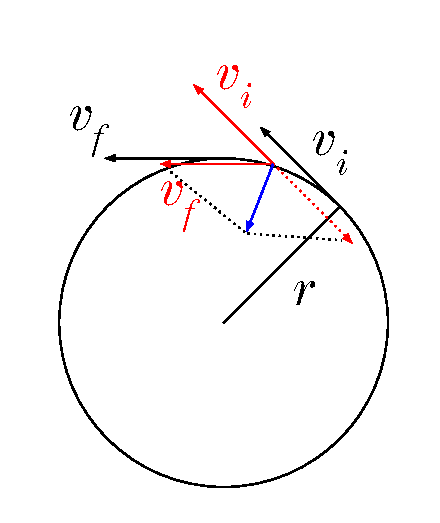
\includegraphics[width = \marginparwidth]{circolare.pdf}
    \caption{Dimostrazione delle caratteristiche geometriche del vettore accelerazione centripeta}
    \label{circolare}
\end{marginfigure}
consideriamo una variazione molto piccola nella posizione angolare dell'oggetto,
che parte con una velocità iniziale $\mathbf{v}_i$ e termina con la
velocità finale $\mathbf{v}_f$, uguali in modulo ma diverse in direzione.
Come già detto, possiamo esprimere l'accelerazione come variazione della
velocità tangenziale.

\[ \mathbf{a} = \frac{d\mathbf{v}}{dt} \simeq \frac{\Delta\mathbf{v}}{\Delta t} \]

\noindent Concentriamoci sul termine $\Delta\mathbf{v}$.

\[ \Delta\mathbf{v} = \mathbf{v}_f - \mathbf{v}_i = \mathbf{v}_f + (-\mathbf{v}_i) \]
Geometricamente, i vettori velocità si sommano secondo la ``regola del parallelogramma''
come mostrato nella Figura. Con i dovuti formalismi geometrici, sapendo che il
modulo di $v$ è sempre costante, possiamo dimostrare che l'accelerazione è
effettivamente centripeta e ortogonale alla velocità tangenziale, ovvero il
suo vettore punta sempre verso il centro della circonferenza. Sempre dalla Figura,
possiamo osservare che al crescere di $v$ cresce anche $a$; tenendo poi
presente che la variazione $\Delta \mathbf{v}$, che è un vettore,
viene moltiplicata per la quantità scalare $\frac{1}{\Delta t}$, il vettore
risultante dell'accelerazione cresce in modulo quanto più piccolo diventa
l'intervallo $\Delta t$: ovvero la velocità dell'oggetto è maggiore.
Dimostreremo più
avanti che la relazione precisa tra i moduli di queste grandezze è data da
\[ a = \frac{v^2}{r} = \omega^2 r \]

\section{Moto armonico}
Supponiamo di osservare un oggetto in moto circolare uniforme, ma invece di
vederlo ``dall'alto'' lo guardiamo con la riconferenza della traiettoria
posta orizzontalmente. Da questo punto di vista, vedremo l'oggetto \textit{oscillare}
a destra e sinistra all'interno di uno spazio la cui larghezza corrisponde al
diametro della circonferenza. Ciò che si vede è un moto particolare, il
\textit{moto armonico semplice}.

Dalla Figura \ref{armonicosemplice} possiamo notare che, fissato il solito
sistema di riferimento $xy$, il moto armonico semplice non è altro che la
proiezione sugli assi di un moto circolare uniforme. Per questo motivo,
possiamo descrivere la posizione dell'oggetto caratterizzato da tale moto:
\begin{marginfigure}
    \centering
    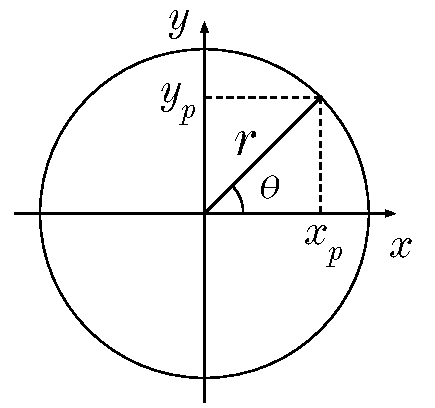
\includegraphics[width = \marginparwidth]{armonico.pdf}
    \caption{Modello di moti armonici semplici a partire da proiezioni
    di un moto circolare uniforme}
    \label{armonicosemplice}
\end{marginfigure}
\[
    \begin{cases}
        x_p(t) = r\cos\theta = r\cos(\omega t)\\
        y_p(t) = r\sin\theta = r\sin(\omega t)
    \end{cases}
\]
Possiamo quindi notare che il moto circolare è la composizione di due moti
armonici.
Sapendo che la velocità corrisponde alla derivata della funzione che
descrive la posizione:
\[
    \begin{cases}
        v_x(t) = -\omega R \sin(\omega t)\\
        v_y(t) = \omega R \cos(\omega t)
    \end{cases}
\]
Derivando nuovamente, otteniamo l'accelerazione:
\[
    \begin{cases}
        a_x(t) = -\omega^2 R\cos(\omega t)\\
        a_y(t) = -\omega^2 R\sin(\omega t)
    \end{cases}
\]
Esiste anche una dimostrazione geometrica di tali relazioni, che non impiega
esplicitamente i metodi del calcolo infinitesimale. È sufficiente tenere in
considerazione la posizione angolare $\theta$, avere dimestichezza con le
funzioni sinusoidali e ricordare direzione e verso dei vettori velocità
tangenziale e accelerazione centripeta durante un moto circolare uniforme.

\subsubsection*{Relazione tra accelerazione centripeta e velocità}
Siamo ora in grado di mostrare l'origine della relazione $a = \frac{v^2}{r} = \omega^2 r$
tra accelerazione centripeta e velocità (angolare e tangenziale) in un moto
circolare uniforme.

Osserviamo che il sistema che descrive l'accelerazione del moto armonico
contiene i termini $r\cos(\omega t)$ e $r\sin(\omega t)$: le coordinate del
punto in moto circolare uniforme in funzione del tempo. Dunque

\[
    \begin{cases}
        a_x(t) = -\omega^2 r\cos(\omega t)\\
        a_y(t) = -\omega^2 r\sin(\omega t)
    \end{cases}
    \Rightarrow
    \begin{cases}
        a_x(t) = -\omega^2 x(t)\\
        a_y(t) = -\omega^2 y(t)
    \end{cases}
\]
Queste non sono altro che le componenti dell'accelerazione centripeta
solidali al sistema di riferimento di assi $xy$. Sapendo che il modulo
di un vettore corrisponde a $|\mathbf{r}| = r = \sqrt{x_r^2 + y_r^2}$
(con $x_r,y_r$ le componenti del vettore $r$ rispetto ad un sistema di
assi ortogonali $xy$), è immediato mostrare che
\[ |\mathbf{a}| = a = \sqrt{(-\omega^2 x)^2 + (-\omega^2 y)^2} = \sqrt{\omega^4x^2 + \omega^4y^2} = \omega^2 \sqrt{x^2 + y^2} = \omega^2 r \]

Dal precedente sistema, è possibile capire perché il vettore dell'accelerazione
è diretto verso il centro della circonferenza: $x$ ed $y$ sono le componenti
del \textit{vettore posizione} dell'oggetto in movimento; tale vettore
non è altro che una freccia di modulo uguale alla lunghezza del raggio e la
cui punta indica il punto in cui il corpo si trova sulla circonferenza,
dunque questo vettore punta verso l'esterno; ma dato che ogni componente
viene moltiplicata per la quantità negativa $-\omega^2$, il vettore
accelerazione centripeta non può che puntare nel verso opposto, quindi
verso il centro della circonferenza. L'equazione vettoriale è dunque la
seguente:
\[ \mathbf{a} = -\frac{\mathbf{v}^2}{\mathbf{r}} \]

\subsubsection*{Accelerazione centripeta, traiettorie curvilinee, raggio di curvatura}
L'accelerazione centripeta non esiste solamente nei moti circolari uniformi,
ma, come possiamo ricordare da esperienze quotidiane, qualsiasi variazione
nella traiettoria di un corpo in moto, attraverso una ``sterzata'', permette
di percepire l'effetto e la direzione dell'accelerazione.
Possiamo dunque estendere la descrizione del moto circolare uniforme a casi
meno eccezionali, come quelli dei moti dalle traiettorie curvilinee. È interessante
come l'equazione dell'accelerazione centripeta permetta di ottenere informazioni
interessantissime su moti come questi, come il \textbf{raggio di curvatura}. Si
osservi l'esempio in Figura \ref{curvilinee}.

\begin{marginfigure}
    \centering
    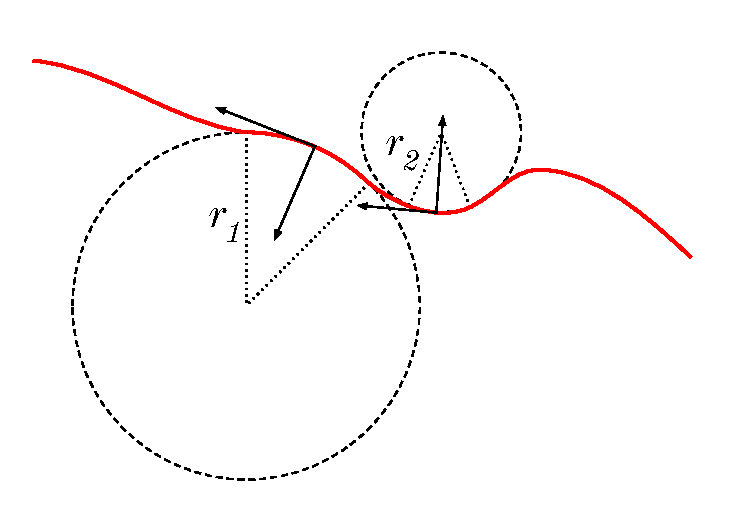
\includegraphics[width = \marginparwidth]{curvilinee.pdf}
    \caption{Una traiettoria curvilinea apporssimata da archi di circonferenze con raggi differenti}
    \label{curvilinee}
\end{marginfigure}

Tratti di traiettorie come queste possono essere approssimate da archi di
circonferenze con raggi di lunghezze differenti. Durante ognuno di questi brevi
tratti, percorsi sugli archi, l'oggetto in moto è sottoposto ad una certa
accelerazione centripeta. Assumento che tale oggetto abbia una massa, è
possibile misurare l'accelerazione rilevando la forza esercitata sull'oggetto
durante il tratto di curva. Dall'equazione dell'accelerazione centripeta,
vale
\[\frac{F}{m} = \frac{v^2}{r}\]
Date le nostre supposizioni sulle grandezze conosciute (forza, massa e velocità), l'unico
dato che rimane è il raggio, che in questo caso prende il nome di
\textit{raggio di curvatura}:
\[ r = \frac{v^2m}{F} \]

\section{Moto nel piano}

\subsubsection*{Parabola di un proiettile}
\[
    \begin{cases}
        x = v_{0,x}t\\
        y = v_{0,y}t - \frac{1}{2}t^2
    \end{cases}
\]
Esprimiamo $y$ in funzione di $x$:
\[
    y = \frac{v_{0,y}}{v_{0,x}}x - \frac{1}{2}\frac{g}{v_{0,x}^2}x^2 = Bx - Cx^2
\]
Tangente a questa parabola:
\[
    y' = B - 2Cx
\]

\subsection{Vettori}
Vettori posizione e spostamento.
\[ \Delta\mathbf{s} = \mathbf{s}_f - \mathbf{s}_i \]

Vettore velocità
\[ \mathbf{v} = \lim_{\Delta t \to 0}\frac{\Delta\mathbf{s}}{\Delta t} = \frac{d\mathbf{s}}{dt} \sim ds\cdot\frac{1}{dt} \]
Per definizione \textit{sempre} tangente alla traiettoria. La traiettoria
è la serie dei punti che si ottiene percorrendo per tratti infinitesimi le
velocità istantanee.

Accelerazione tangente e accelerazione normale.


\subsubsection*{Esercizio}
$|\mathbf{v}_i| = 50\text{ km/h}$, $|\mathbf{v}_f| = 100\text{ km/h}$,
$m = 1800\text{ kg}$, $R = 20\text{ m}$, $\Delta t = 2\text{ s}$. $|\mathbf{F}_n| = ?$ (forza normale),
$|\mathbf{a}_t| = ?$. Assumiamo che l'auto acceleri con costanza tra le
due velocità.

\begin{itemize}
    \item $a_{n,i} = \frac{v_i^2}{R}$, $a_{n,f} = \frac{v_f^2}{R}$
    \item $F_{n,i} = ma_{n,i} \simeq 17100 \text{ N}$, $F_{n,f} = ma_{n,f} \simeq 68400\text{ N}$
    \item $|\mathbf{a}_t| = \textit{cost} = \frac{|\Delta\mathbf{v}|}{\Delta t} \simeq 6,95\text{ m/s}^2$
\end{itemize}


\section*{Recap}
\[ \mathbf{x} = \mathbf{x_0} + \mathbf{v}(t - t_0) \]
Semplificazioni in termini di variazioni, infinità.
% Lezione 3/2024-03-04
% - introduzione alla dinamica
% - prima e seconda legge
% - esercizi su moto uniformemente accelerato
% - accenni al concetto di forza e introduzione alla forza elastica con legge di hooke

% Lezione 4/2024-03-06
% - grafico orario: grafico nel quale un asse riporta lo spazio (una dimensione), mentre sull'altro il tempo
% - differenza tra SPOSTAMENTO e distanza
% - interpretazione grafica della velocità e accelerazione, con analisi di funzione

\chptr{Dinamica}
\marginpar{\minitoc}

\section{Recap}
\[ \overrightarrow{x} = \overrightarrow{x_0} + \overrightarrow{v}(t - t_0) \]
Semplificazioni in termini di variazioni, infinità.

\section{Leggi della dinamica}

Nella descrizione introduttiva del moto, non è stata analizzata alcuna causa del
fenomeno.

\subsection{La prima legge}

\vspace{8pt}
\begin{tcolorbox}[colback = red!30, colframe = red!30!black, title = {Prima legge della dinamica (legge di inerzia)}]
    Un corpo permane nel suo stato di \textit{quiete} o moto rettilineo uniforme
    finché non intervenga un \textit{agente esterno}.
\end{tcolorbox}
\vspace{5pt}

In altre parole, se nulla ``rompe le scatole'' al corpo, esso permanerà nel suo
stato di moto, naturalmente.

\vspace{8pt}
\begin{tcolorbox}[colback = yellow!30, colframe = yellow!30!black, title = {Sistema inerziale}]
    Sistema nel quale vale la prima legge della dinamica.
\end{tcolorbox}
\vspace{5pt}

\subsection{La seconda legge}
Quando l'agente esterno agisce sull'oggetto, l'effetto è un cambiamento nello
stato di moto di quell'oggetto. Ovvero, cambia la sua velocità. La variazione
della velocità nel tempo è chiamata \textbf{accelerazione}.

\[ \lim_{\Delta t \to 0} \frac{\Delta v}{\Delta t} = \frac{dv}{dt} = a \]

\vspace{8pt}
\begin{tcolorbox}[colback = red!30, colframe = red!30!black, title = {Seconda legge della dinamica}]
    \begin{align}
        \frac{|\overrightarrow{F}|}{|\overrightarrow{a}|} = \frac{F}{a} = m
    \end{align}
\end{tcolorbox}
\vspace{5pt}


Gli oggetti hanno inerzia, ovvero capacità di opporsi all'agire dell'agente
esterno. Questa capacità di opporsi è rappresentato da una quantità detta
massa (inerziale).

\subsection{Analisi dimensionale}
\[ [F] = [ma] = \left[m\cdot\frac{v}{t}\right] = \left[m\cdot\frac{l}{t^2}\right]  \]
\[ 1\text{ kg}\cdot\frac{\text{m}}{\text{s}^2} = \text{udm}\left[M\cdot\frac{L}{T^2}\right] = \text{udm}[F] = 1\text{ N} \]


\subsection{Molla e forza elastica}
\[ F \propto \Delta x \]

La forza che la molla esercita, essendo in opposizione alla direzione nella
quale la deformazione viene effettuata, corrisponde a:
\[ F_\textit{el} = -k\Delta x \]

\section{Forza agente sul moto}
Un blocco di massa $m = 10 \text{ kg}$ viaggia ad una velocità $v_i =
2 \text{ m/s}$. Una forza $F = 20 \text{ N}$ agisce sul blocco per
$T = 5 \text{ s}$. Quale velocità raggiungerà il blocco dopo $T$?.
Dopo $T$, la forza cessa di agire e il blocco viaggia a $v_f$ trovata
precedentemente. Includendo lo spazio percorso durante $T$ (e dunque il
tempo $T$), quanto tempo impiega il blocco a coprire $s_w = 2\text{ km}$
di distanza?

\begin{marginfigure}
    \centering
    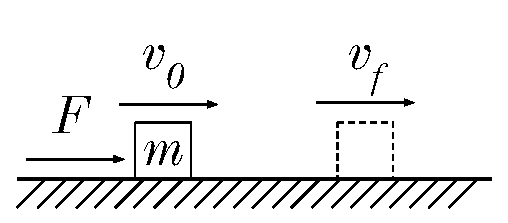
\includegraphics[width = \marginparwidth]{figures/scivola.pdf}
    \caption{Forza agente su una massa in moto}
\end{marginfigure}

Per rispondere al primo quesito, possiamo assumere un moto rettilineo
uniformemente accelerato durante l'intervallo $T$. Sappiamo che \[ a = \frac{F}{m} = \frac{dv}{dt} \]
Da cui possiamo esprimere la velocità in funzione del tempo (la velocità
iniziale la conosciamo già, ma assumiamo un tempo iniziale $t_0 = 0$):
\[ \frac{F}{m}dt = dv \to \int_{t_0}^{t}\frac{F}{m}dp = \int_{v_0}^{v}dw \to \frac{F}{m}\int_{0}^{t}dp = v - v_0 \to \frac{F}{m}t = v - v_0 \]
Dunque
\[ v(t) = v_0 + \frac{F}{m}t \]
Non ci manca che calcolare la velocità in corrispondenza di un $t_f = t_0 + \Delta t = 0 + T = T$:
\[ v(t_f) = v(T) = v_0 + \frac{F}{m}T \]

Nel secondo quesito, possiamo spezzare il problema in due parti: durante
l'azione della forza, la distanza percorsa ($s_a$) deve essere calcolata tenendo
conto del moto uniformemente accelerato, mentre nell'intervallo di tempo
successivo ($T_v$) il moto è semplicemente uniforme. Dalla seguente equazione,
possiamo ricavare $T_v$ ($T$ lo conosciamo già).
\[ s_w = s_a + s_v = s_a + v_fT_v = \int_{0}^{T}(v_0 + at)dp + v_fT_v = v_0T + \frac{1}{2}aT^2 + v_fT_v \]
Il tempo per percorrere $2\text{ km}$ è dunque:
\[ T_{2\text{ km}} = T + \frac{s_w - v_iT - \frac{F}{2m}T^2}{v_f} = T + \frac{s_w - v_iT - \frac{F}{2m}T^2}{v_i + \frac{F}{m}T} \]

\section{Lancio verso l'alto}
Si consideri la situazione mostrata in Figura \ref{lanciobasso}.
Durante la salita, l'oggetto rallenta a causa dell'accelerazione di gravità $g$.
Determiniamo la quota che l'oggetto raggiungerà.

\[ a = \frac{dv}{dt} \to dv = adt \to \int_{v_0}^{v}dw = \int_{t_0}^{t}adp \to v - v_0 = a\int_{t_0}^{t}dp \to v - v_0 = a(t - t_0) \]
Dunque
\[ v(t) = v_0 + a(t - t_0) = v_0 + at \]
Rallentando, si arriverà ad un istante $t_f$ nel quale l'oggetto avrà velocità
nulla:
\begin{marginfigure}
    \centering
    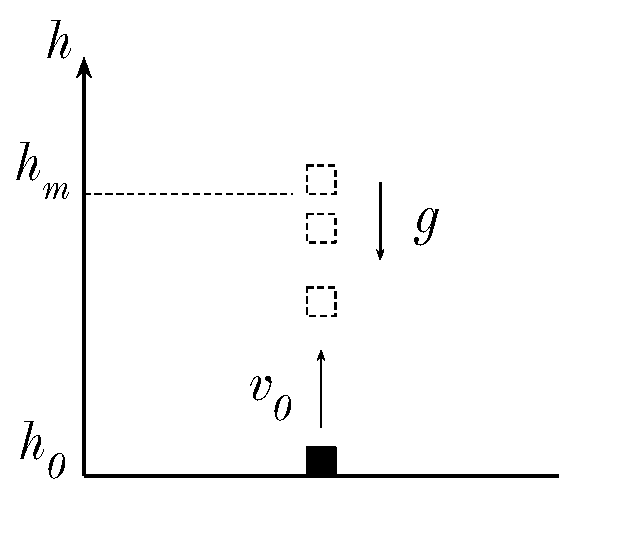
\includegraphics[width = \marginparwidth]{figures/greve.pdf}
    \caption{Lancio di un oggetto verso l'alto}
    \label{lanciobasso}
\end{marginfigure}
\[ v(t_f) = 0 \to v_0 + at_f = 0 \]
Non disponiamo tuttavia del tempo, ma possiamo avvalerci della legge oraria
che descrive la distanza percorsa:
\[ v(t) = \frac{dh}{dt} \to \int_{h_0}^{h}dk = \int_{t_0}^{t}v(t)dp \to h - h_0 = \int_{t_0}^{t}(v_0 + ap)dp \]
\[ h - h_0 = v_0\int_{t_0}^{t}dp + a\int_{t_0}^{t}pdp \to h - h_0 = v_0t + \frac12 at^2 \]
Da cui:
\[ h(t) = h_0 + v_0t + \frac12 at^2 = v_0t + \frac12 at^2 \]
Abbiamo quindi ottenuto la quota in funzione del tempo, che possiamo ricavare
dall'equazione $v_0 + at_f = 0 \to t_f = -\frac{v_0}{a}$.
\[ h(t_f) = v_0t_f + \frac12 at_{f}^2 =  -\frac{v_0^2}{a} + \frac{1}{2}a\frac{v_0^2}{a^2} = -\frac{v_0^2}{a} + \frac{v_0^2}{2a} = -\frac{v_0^2}{2a} \]
Sapendo che $a = -|g|$, la quota massima $h_m$ raggiunta è:
\[ h_m = \frac{v_0^2}{2|g|} \]

%%%%%%%%%%%%%%%%%%%%%%%%%%%%%%%%%%%%%%%%%%%%%%%%%%%%%%%%%%%%%%%%%

\subsection*{Spostamento}
\[ \Delta\overrightarrow{s} = \overrightarrow{s}_f - \overrightarrow{s}_i \]


\subsection{La terza legge}
\vspace{8pt}
\begin{tcolorbox}[colback = red!30, colframe = red!30!black, title = {Terza legge della dinamica}]

\end{tcolorbox}
\vspace{5pt}



\vspace{8pt}
\begin{tcolorbox}[colback = red!30, colframe = red!30!black, title = {Accelerazione centripeta nel moto circolare uniforme}]
\begin{align}
    a = \frac{v^2}{r} = \omega^2 r
\end{align}
\end{tcolorbox}
\vspace{5pt}

\chptr{Meccanica}
\marginpar{\minitoc}

\section{Lavoro di una forza}


Il lavoro di una forza costante corrisponde al prodotto scalare\footnote{Ricordiamo
che il prodotto scalare $p$ tra due vettori \textbf{a} e \textbf{b} è un valore scalare
definito da $p = |\textbf{a}||\textbf{b}|\cos\theta_{\textbf{ab}}$, con $\theta_\textbf{ab}$
l'angolo tra i vettori.}
tra la forza e lo spostamento:
\begin{align}
W = \textbf{F}\cdot\textbf{r}
\end{align}
Il lavoro si misura in Joule (J), dove
\[ 1\text{ J} = 1\text{ Nm} = 1\text{ kg$\frac{\text{m}^2}{\text{s}^2}$} \]


Lavoro di una forza variabile durante lo spostamento:
\begin{align}
    W_{AB} = \int_{A}^{B}\textbf{F}(r)\cdot d\textbf{r}
\end{align}

\section*{app}
Si parte da $\overrightarrow{F} = m\overrightarrow{a} \Rightarrow
\overrightarrow{F} = m\frac{d\overrightarrow{v}}{dt}$. Abbiamo una traiettoria
qualsiasi, posizione descritta da $\overrightarrow{r}(t)$. Prendiamo una variazione
infinitesima della posizione $\Delta\overrightarrow{r}\to d\overrightarrow{r} =
\overrightarrow{r}_f - \overrightarrow{r}_i$.

\subsection{Lavoro di una forza}
\[ dW = \textbf{F}\cdot d\textbf{r} = |\textbf{F}||d\textbf{r}|\cos\theta \]
Può essere positivo, negativo, nullo.
\begin{itemize}
    \item \textbf{Lavoro motore} $dW > 0$
    \item \textbf{Lavoro resistente} $dW < 0$ (la forza si oppone allo spostamento)
    \item \textbf{Lavoro nullo} $dW = 0$ (la forza è ortogonale allo spostamento),
    es forza centripeta
\end{itemize}

Analisi dimensionale:
\[ \left[dW\right] = \left[\textbf{F}d\textbf{r}\right] = \left[M\frac{L}{T^2}L\right] = \left[M\left(\frac{L}{T}\right)^2\right] \]
\[ 1\text{ J} = 1\text{ Nm} = 1\text{ kg$\frac{\text{m}^2}{\text{s}^2}$} \]

Esempio cammino sentiero
\[ W_{A\to B} = \sum_{i = A}^{N = B}dW_i \to \int_{A}^{B}dW \text{ per } N\to\infty \]
\[ W_{A\to B} = \int_{A}^{B}\textbf{F}\cdot d\textbf{r} \]
Notiamo che 
\[ \textbf{P}\cdot d\textbf{r} = |\textbf{P}| (|d\textbf{r}|\cos\theta) \]
Dove abbiamo la proiezione dello spostamento sul peso P. Questo significa che
per calcolo del lavoro importa solo la variazione della quota, $dh$.
\[ W_{0\to 2000\text{ m}} = \sum_{0}^{2000}\textbf{P}\cdot d\textbf{r} = \int_{0}^{2000}mg dh = mgh_{bondone} \]

\subsubsection*{Versore}
\[ \hat{v} = \frac{\overrightarrow{v}}{|\overrightarrow{v}|} \]

\[ W = \int_{i}^{f}\overrightarrow{F}\cdot d\overrightarrow{s} = \int_{0}^{L}(F\hat{f})\cdot(ds\hat{x}) = F(\hat{f}\cdot\hat{x})\int_{0}^{L}ds = F\cos(\theta) L\]
Quindi
\[ \cos\theta = \frac{W}{FL} \]

\section{Teorema delle forze vive}
\textit{vis viva} (forza viva), quantità che viene dalle forze, che pareva avere
vita propria, in grado di trasferirsi da corpo a corpo.
Partiamo da seconda legge della dinamica
\[ \textbf{F} = m\frac{d\textbf{v}}{dt} \]
Senza giustificare le ragioni matematiche dei prossimi passaggi, ma facendoci
guidare dall'intuizione fisica, eseguiamo il prodotto scalare con $d\textbf{s}$
su entrambi i membri
\[ \textbf{F}\cdot d\textbf{s} = m\frac{d\textbf{v}}{dt}\cdot d\textbf{s} = m d\textbf{v}\cdot\frac{d\textbf{s}}{dt} \]
Notiamo che questa operazione ha permesso di ottenere un lavoro al membro di
sinistra, mentre a destra si ottiene il termine $d\mathbf{s}/dt$, che corrisponderebbe
proprio alla velocità $\textbf{v}$. Con ulteriori sviluppi, si raggiunge la
seguente equazione (il simbolo $d$ ha il significato fisico di variazione o
differenza infinitesima).
\[ \textbf{F}\cdot d\textbf{s} = m\textbf{v}\cdot d\textbf{v} = m\text{ }d\left[\frac{v^2}{2}\right] \]
Dimostriamo come sviluppare il termine $\textbf{v}\cdot d\textbf{v} = d\left[\frac{v^2}{2}\right]$.
Ricorriamo alla definizione vettoriale di prodotto scalare\footnote{Il prodotto scalare
di due vettori \textbf{a} e \textbf{b} è calcolabile anche attraverso la somma
dei prodotti tra i valori delle componenti dei due vettori: $\mathbf{a}\cdot\mathbf{b} = a_xb_x + a_yb_y + ...$}
e utilizziamo questo abuso di notazione, ma ragionevole dal punto di vista fisico:
\[ \int x \,dx =  \frac{x^2}{2} + c \Rightarrow \frac{d}{dx}\left[\frac{x^2}{2} + c\right] = x \Rightarrow \int x \,dx = \int d\left[\frac{x^2}{2}\right] \]
Quindi
\[ v_x dv_x + v_y dv_y + v_z dv_z \Rightarrow d\left[\frac{v_x^2}{2}\right] + ... = d\left[\frac{v_x^2 + ...}{2}\right] = d\left[\frac{v^2}{2}\right] \]
Riprendendo l'equazione $\mathbf{F}\cdot d\textbf{s} = m\text{ }d\left[\frac{v^2}{2}\right]$ otteniamo
\[ dW = d\left[\frac12 mv^2\right] \]
Il termine $E_K = \frac{1}{2}mv^2$ viene chiamato \textit{energia cinetica}. Quindi
\[ dW = dE_K \]
Questa equazione può essere tradotta come ``una infinitesima quantità di lavoro
corrisponde ad una variazione infinitesima dell'energia cinetica''. Ora possiamo
enunciare il teorema delle foze vive:
\vspace{8pt}
\begin{tcolorbox}[colback = red!30, colframe = red!30!black, title = {Teorema dell'energia cinetica (o delle forze vive)}]
    Quando una forza (risultante) applicata a un oggetto per un dato tratto di
    traiettoria, compie su di esso un lavoro, il risultato è una variazione del
    modulo della velocità dell'oggetto e quindi una variazione della sua energia
    cinetica. Quindi, il lavoro compiuto su un oggetto è uguale alla variazione
    della sua energia cinetica.
    \begin{align}
        W_{i\to f}^{(R)} = E_{K,f} - E_{K,i}
    \end{align}
\end{tcolorbox}
\vspace{5pt}

\noindent È necessario sottolineare alcune osservazioni:
\begin{enumerate}
    \item Il teorema presuppone che il lavoro sia dovuto all'effetto della risultante delle forze agenti sul corpo.
    \item Il lavoro è rappresentato da una variazione di energia cinetica. Possiamo descrivere dunque lo stato finale
    come \[ E_{K,f} = E_{K,i} + W_{i\to f} \] dunque se il lavoro, quindi l'energia trasferita all'oggetto, è positivo,
    l'energia cinetica aumenta e viceversa.

    \item Il teorema sposta la descrizione del sistema fisico dal piano vettoriale a quello scalare. Ovvero, partendo
    da grandezze vettoriali, abbiamo ottenuto una legge dove compaiono solamente dei numeri. Ciò rende particolarmente agevole
    l'utilizzo del teorema in svariati problemi nei quali l'analisi vettoriale può essere ostica.

    \item Il teorema è molto potente per la sua validità generale, perché non sono state fatte ipotesi sulla natura delle
    forze, se non presupponendo come vera la seconda legge della dinamica $\textbf{F} = m\textbf{a}$.
\end{enumerate}

\subsubsection*{Applicazione del teorema delle forze vive}
Supponiamo di avere un punto di massa $m$ sulla sommità di un piano inclinato di
alteza $h$ con
un angolo $\theta$ rispetto all'orizzontale. Sappiamo che la massa parte dalla
cima con velocità $v_i$ parallela alla lunghezza del piano e diretta verso la
discesa. Vogliamo trovare la velocità finale della massa. Si esprima il calcolo sia
con che senza attrito, considerando nell'ultimo caso un coefficiente di attrito
dinamico $\mu$.
\[ W = \Delta E_K \]
\[ W = \mathbf{P}\cdot\mathbf{L} = |\mathbf{P}||\mathbf{L}|\cos\left(\frac{\pi}{2} - \theta\right) = |\mathbf{P}||\mathbf{L}|\sin\theta = |\mathbf{P}|h = mgh \]
\[ \Delta E_K = \frac12mv_f^2 - \frac12mv_i^2 \]
Quindi
\[ mgh = \frac12mv_f^2 - \frac12mv_i^2 \]
\[ v_f = \sqrt{2gh + v_i^2} \]

Con attrito il peso è contrastato. L'attrito compie il suo lavoro per tutta la
lunghezza del piano fino alla fine della discesa. L'espressione della differenza
di energia cinetica è tuttavia la stessa.
\[ W = W_P - W_A = Ph - F_AL = Ph - \mu F_\perp L = mgh - \mu mg\sin\theta L \]


%\chptr{Lezione 2024-02-26}
%\section*{Riassunto}
%\begin{itemize}
%    \item Dinamica: dinamica del punto materiale (3 leggi dinamica)
%    \item Meccanica: quantita' conservative (energia ecc)
%    \item Termodinamica dei gas
%    \item Entropia/probabilita'/senso del tempo
%    \item Elettricita': Coulomb
%    \item Magnetismo
%\end{itemize}

%\setcounter{chapter}{0}

%\part{Esercitazioni}
%\chptr{Dinamica}
\section{Masse collegate su un piano inclinato}
Due blocchi sono collegati per mezzo di una corda, come in Figura \ref{primo}.
Il blocco che si trova sulla superficie liscia e inclinata di $35$° rispetto
all'orizzontale ha massa $m_1 = 5,7\text{ kg}$. La massa del blocco appeso
è $m_2 = 3,2\text{ kg}$. Determinare il modulo e il verso dell'accelerazione
del blocco appeso.
\begin{marginfigure}
    \centering
    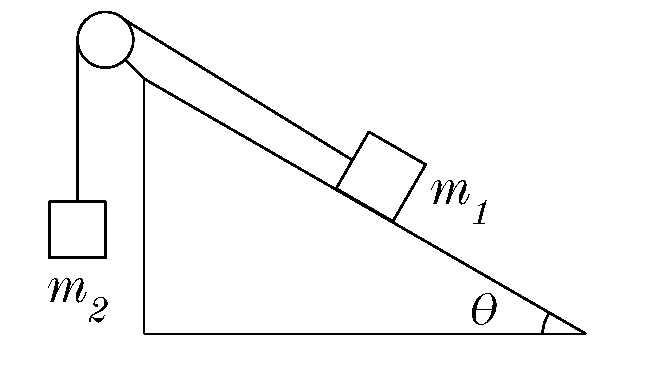
\includegraphics[width = \marginparwidth]{figures/carrucolainclinata.pdf}
    \caption{Piano inclinato molto interessante}
    \label{primo}
\end{marginfigure}
\\\\
\noindent Soluzione:

\section{Tensione delle corde}

\part{Appendici}
\section*{Link utili}
\begin{itemize}
    \item \href{https://drive.google.com/drive/folders/1nu4RMBqniPuS5pC0v9kfnmJ1coKzccGm?usp=sharing}{\textcolor{blue}{Immagini}}
\end{itemize}

\end{document}